\section{Results}
\frametitle{Results}
    \begin{frame}{Results}
        \begin{itemize}
            \item The main arm has \theta_{1}=1.649 rad,
            \theta_{2}=1.475-2.617 rad.
        \end{itemize} 
        \begin{columns}
            \begin{column}{0.5\textwidth}
                \begin{figure}
                \centering
                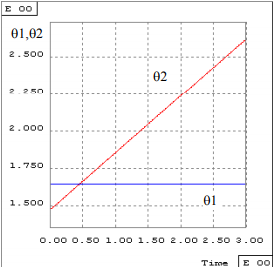
\includegraphics[width=.8\textwidth]{fig/cond1.png}
                \caption{Input angles.}
                \end{figure}
            \end{column}
        
            \begin{column}{0.5\textwidth}
                \begin{figure}
                \centering
                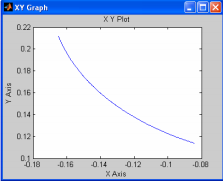
\includegraphics[width=.8\textwidth]{fig/fig1.png}
                \caption{Output variables(final position).}
                \end{figure}
            \end{column}
        \end{columns}
    \end{frame}

    \begin{frame}{Results}
        \begin{itemize}
            \item The main arm has \theta_{1} = 3.0142-0.794 rad, \theta_{2}= 2.449 rad.
        \end{itemize} 
        \begin{columns}
            \begin{column}{0.5\textwidth}
                \begin{figure}
                \centering
                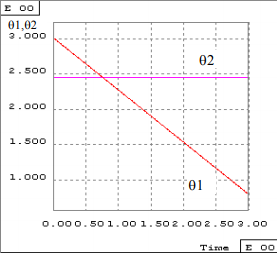
\includegraphics[width=.8\textwidth]{fig/cond2.png}
                \caption{Input angles.}
                \end{figure}
            \end{column}
        
            \begin{column}{0.5\textwidth}
                \begin{figure}
                \centering
                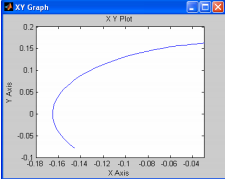
\includegraphics[width=.8\textwidth]{fig/fig2.png}
                \caption{Output variables(final position).}
                \end{figure}
            \end{column}
        \end{columns}
    \end{frame}

    \begin{frame}{Results}
        \begin{itemize}
            \item The main arm has \theta_{1} = 0.232-2.469 rad,
            \theta_{2}= 1.352 - 2.094 rad.
        \end{itemize} 
        \begin{columns}
            \begin{column}{0.5\textwidth}
                \begin{figure}
                \centering
                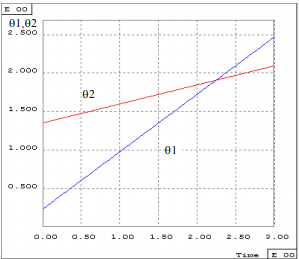
\includegraphics[width=.8\textwidth]{fig/cond3.png}
                \caption{Input angles.}
                \end{figure}
            \end{column}
        
            \begin{column}{0.5\textwidth}
                \begin{figure}
                \centering
                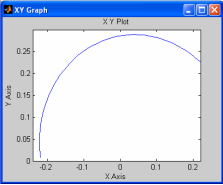
\includegraphics[width=.8\textwidth]{fig/fig3.png}
                \caption{Output variables(final position).}
                \end{figure}
            \end{column}
        \end{columns}

    \end{frame}

